\documentclass[oneside]{scrbook}
\usepackage{syntax}
\usepackage{hypernat}
\usepackage[hidelinks]{hyperref}
\usepackage{color}
\usepackage{booktabs}
\usepackage{multirow}
\usepackage{multicol}
\usepackage{amsmath}
\usepackage{xspace}
\usepackage{pgf}
\usepackage{tikz}
\usepackage{comment}
\usepackage{xifthen}
\usepackage{listings}
\usepackage{courier}
\usepackage{newfloat}
\usepackage{fancyvrb}

\makeatletter
\makeatother

\usetikzlibrary{shapes}
\usetikzlibrary{snakes}
\usetikzlibrary{patterns}
\usetikzlibrary{circuits}
\usetikzlibrary{arrows}
\usetikzlibrary{calc}
\usetikzlibrary{fit}

\let\ab\allowbreak

\definecolor{codegreen}{rgb}{0,0.6,0}
\definecolor{codegray}{rgb}{0.5,0.5,0.5}
\definecolor{codepurple}{rgb}{0.58,0,0.82}
\definecolor{backcolour}{rgb}{0.95,0.95,0.92}
\definecolor{darkmagenta}{rgb}{0.55,0,0.55}

\newcommand{\uclid}{{\textsc{Uclid5}}\xspace}
\newcommand{\keyword}[1]{\textcolor{darkmagenta}{\texttt{#1}}}
\newcommand{\ident}[1]{\textcolor{black}{\texttt{#1}}}
\newcommand{\keywordbf}[1]{\textcolor{darkmagenta}{\texttt{{#1}}}}
\newcommand{\proofcmd}[1]{\textcolor{blue}{\texttt{{#1}}}}
\newcommand{\codelike}[1]{\texttt{#1}}

\DeclareFloatingEnvironment[fileext=frm,name={Example},listname={List of \uclid{} Examples}]{uclidlisting}

\lstdefinelanguage{uclid}{
  sensitive = true,
  keywords={module, forall, exists, Lambda, if, else, assert, assume, havoc,
            for, range, skip, case, esac, init, next, control, function, procedure,
            returns, call, define, type, var, input, output, const, property,
            invariant, synthesis, grammar, requires, ensures, modifies, instance, axiom, 
            enum, record, integer, boolean, true, false, group, oracle},
 %otherkeywords={% types
 %   integer, boolean, true, false,
 %   bv1, bv2, bv3, bv4, bv5, bv6, bv7, bv8, bv9, bv10, bv11, bv12, bv13, bv14, bv15, 
 %   bv16, bv17, bv18, bv19, bv20, bv21, bv22, bv23, bv24, bv25, bv26, bv27, bv28, bv29, bv30, bv31, 
 %   bv32, bv33, bv34, bv35, bv36, bv37, bv38, bv39, bv40, bv41, bv42, bv43, bv44, bv45, bv46, bv47, 
 %   bv48, bv49, bv50, bv51, bv52, bv53, bv54, bv55, bv56, bv57, bv58, bv59, bv60, bv61, bv62, bv63
 %   %>, <, ==, <=, >=, +, -, *, !=
 %},
  numbers=left,
  numberstyle=\scriptsize,
  stepnumber=1,
  numbersep=8pt,
  showstringspaces=false,
  breaklines=true,
  frame=top,
  comment=[l]{//},
  morecomment=[s]{/*}{*/},
}

\definecolor{codegreen}{rgb}{0,0.6,0}
\definecolor{codegray}{rgb}{0.5,0.5,0.5}
\definecolor{codepurple}{rgb}{0.58,0,0.82}
\definecolor{backcolour}{rgb}{1.0,1.0,1.0}

\lstdefinestyle{uclidstyle}{
  backgroundcolor=\color{backcolour},
  commentstyle=\color{codegreen},
  keywordstyle=\color{magenta},
  numberstyle=\tiny\color{codegray},
  stringstyle=\color{codepurple},
  basicstyle=\footnotesize,
  breakatwhitespace=false,
  basicstyle=\footnotesize\ttfamily,
  breaklines=true,
  captionpos=b,
  keepspaces=true,
  numbers=left,
  numbersep=5pt,
  showspaces=false,
  showstringspaces=false,
  showtabs=false,
  tabsize=2,
  frame=shadowbox
}

\begin{document}
\title{Getting Started with {\uclid}\\}
\author{Pramod Subramanyan, Sanjit A. Seshia \footnote{with contributions from Demetris Christodoulou, Kevin Cheang, Federico Mora and Elizabeth Polgreen} \\
        \textit{\{spramod, sseshia\}@eecs.berkeley.edu}}
\date{November 2021}
\maketitle

\tableofcontents
\listofuclidlisting

\chapter{Introduction}

\uclid{} is a software toolkit for the formal modeling, specification,
verification, and synthesis of computational systems. 
The \uclid{} toolchain aims to:
\begin{enumerate}
\item Enable compositional (modular) modeling of finite and infinite state transition systems across a range of concurrency models and background logical theories;
\item Verification of a range of properties, including assertions, invariants, and temporal properties, and % mention hyperproperties in a future release
\item Integrate modeling and verification with algorithmic and inductive synthesis.
\end{enumerate}

\uclid draws inspiration from the earlier {UCLID} system for modeling
and verification of systems~\cite{bryant-cav02,DBLP:conf/cav/LahiriS04}, in particular
the idea of modeling concurrent systems in first-order logic 
with a range of background theories, and the use of proof scripts
within the model. However, the \uclid modeling
language and verification capabilities go beyond the original modeling 
language, and the planned integration with synthesis is novel.

This document serves as introduction to the \uclid{} modeling 
language and toolchain. With the \uclid system under active
development, we expect this document to undergo several changes
as the system and its applications evolve.

\section{Getting Started: A Simple \uclid{} Model}

\begin{uclidlisting}[htbp]
    \lstinputlisting[language=uclid,style=uclidstyle]{../examples/tutorial/ex1.1-fib-model.ucl}
    \label{ex:fib-model}
\caption{A \uclid{} model that computes the Fibonacci sequence}
\end{uclidlisting}

A simple \uclid{} module that computes the Fibonacci sequence is shown in Example~\ref{ex:fib-model}.  We will now walk through each line in this model to understand the basics of \uclid{}.

The top-level syntactic structure in \uclid{} is a \keywordbf{module}. All modeling, verification and synthesis code in \uclid{} is contained within modules. In Example~\ref{ex:fib-model}, we have defined one \keyword{module} named \ident{main}. This module starts on line 1 and ends on line 18. The module can be conceptually split into three parts: a system model, a specification and proof script. 

In the example, these three conceptual parts are also kept separate in the code.\footnote{This is not required by \uclid{} syntax, as \keywordbf{invariant} declarations and assumptions can be interleaved with \keyword{init}, \keyword{next}, \keyword{var} declarations as well other types of declarations. However, keeping these conceptually different parts separate is good design practice. \uclid{} does require that if a \keyword{control} block is specified, then it is the very last element of a module.} The following subsections will describe each of these sections of the module. 

\subsubsection{The System Model}
This part of a \uclid{} module describes the functionality of the transition system that is being modeled: it tells us \emph{what the system does}.

The first item of interest within the module \ident{main} are \emph{state variables}. These are declared using the \keywordbf{var} keyword. The module \ident{main} declares two state variables: \ident{a} and \ident{b} on line~3. These are both of type \keywordbf{integer}, which corresponds to mathematical integers.\footnote{Mathematical integer types, as opposed to the machine integer types present in languages like C/C++ and Java, do not have a fixed bit-width and do not overflow.}

The \keywordbf{init} block appears next and spans lines 5 to 8. It defines the initial values of the state variables in the module. The notation \codelike{a'} refers to the value of the state variable \ident{a} at the end of the current ``step'', which in this case refers to initial state. The model is specifying that after the \codelike{init} block is executed, \codelike{a} and \codelike{b} have the values 0 and 1 respectively.

The \keywordbf{next} block appears after this and it defines the transition relation of the module. In the figure, the next statement spans from lines 9 to 11; \ident{a} is assigned to the (old) value of \ident{b}, while b is assigned to the value \ident{a} + \ident{b}.

\subsubsection{The System Specification}
The specification answers the question: \emph{what is the system supposed to do?}. 

In our example, we have a single \keywordbf{invariant} that comprises that entire specification. Line 14 defines this \keyword{invariant}. It is named \ident{a\_le\_b} and as the name suggests, it states that \ident{a} must be less than or equal to \ident{b} for every reachable state of the system.

\subsubsection{The Proof Script}
The third and final part of the \uclid{} module is a set of commands to the \uclid{} verification engine. These tell how we should go about proving\footnote{We are using a broad definition of the word ``prove'' here to refer to any systematic method that gives us assurance that the specification is satisfied.} that the system satisfies its specification.

The proof script is contained within the \keywordbf{control} block. The commands here execute the system for 3 steps and check whether all of the systems properties (in this case, we only have one invariant: \ident{a\_le\_b}) are satisfied for each of these steps. 

The command \proofcmd{bmc} executes the system for 3 steps. This execution generates four \emph{proof obligations}. These proof obligations ask whether the system satisfies the invariant \ident{a\_le\_b} in the initial state and in each of the 3 states reached next. The \proofcmd{check} command \emph{checks} whether these proof obligations are satisfied and the \proofcmd{print\_results} prints out the results of these checks.

\section{Installing \uclid{}}

Public releases of the \uclid{} can be obtained at: \url{https://github.com/uclid-org/uclid/releases}. For the impatient, the short version of the installation instructions is: download the archive with the latest release, unzip the archive and add the `bin/' subdirectory to your \codelike{PATH}. 

More detailed instructions for installation are as follows.

\subsection{Prerequisites}

\uclid{} has two prerequisites. 
\begin{enumerate}
    \item \uclid{} requires that the Java\texttrademark{} Runtime Environment be installed on your machine. You can download the latest Java Runtime Environment for your platform from \url{https://www.java.com}. 
\item \uclid{} uses the Z3 SMT solver. You can install Z3 from: \url{https://github.com/Z3Prover/z3/releases}. Make sure the `z3' or `z3.exe' binary is in your path after Z3 installed. Also make sure, the shared libraries for libz3 and libz3java are in the dynamic library load path (\codelike{LD\_LIBRARY\_PATH} on Unix-like systems).
\end{enumerate}

\uclid{} has been tested with Java\texttrademark{} SE Runtime Environment version 1.8.0 and Z3 versions 4.5.1 and 4.6.0.

\subsection{Detailed Installation Instructions}

First, down the platform independent package from \url{https://github.com/uclid-org/uclid/releases}.

Next, follow these instructions which are provided for the bash shell running on a Unix-like platform. Operations for Micosoft Windows, or a different shell should be similar.

\begin{itemize}
  \item Unzip the archive.

  \codelike{\$ unzip uclid-0.9.5.zip}.

\begin{comment}
  This should produce output similar to the following.
\begin{Verbatim}[frame=single]
Archive:  uclid-0.9.5.zip
  inflating: uclid-0.9.5/lib/default.uclid-0.9.5.jar  
  inflating: uclid-0.9.5/lib/com.microsoft.z3.jar  
  inflating: uclid-0.9.5/lib/org.scala-lang.scala-library-2.12.0.jar  
  inflating: uclid-0.9.5/lib/org.scala-lang.modules.scala-parser-combinators_2.12-1.0.6.jar  
  inflating: uclid-0.9.5/lib/org.scalactic.scalactic_2.12-3.0.1.jar  
  inflating: uclid-0.9.5/lib/org.scala-lang.scala-reflect-2.12.0.jar  
  inflating: uclid-0.9.5/bin/uclid     
  inflating: uclid-0.9.5/bin/uclid.bat  
\end{Verbatim}
\end{comment}


  \item Add the \codelike{uclid} binary to your path.

  \codelike{\$ export PATH=\$PATH:\$PWD/uclid-0.9.5/bin/}

  \item Check that the \texttt{uclid} works.

  \codelike{\$ uclid}

  This should produce output similar to the following.
\begin{Verbatim}[frame=single, samepage=true]
$ uclid

    Usage: uclid [options] filename [filenames]
    Options:
      -h/--help : This message.
      -m/--main : Set the main module.
      -d/--debug : Debug options.
  
Error : Unable to find main module.
\end{Verbatim}
\end{itemize}

\subsection{Running \uclid{}}

Invoke \uclid{} on a model is easy. Just run the \codelike{uclid} binary and provide a list of files containing the model as a command-line argument. When invoked, \uclid{} will parse each of these files and look for a module named \codelike{main} among them. It will execute the commands in the \codelike{main} module's control block. The \codelike{--main} command line argument can be used to specify a different name for the ``main'' module. Note only the \codelike{main} module's control blocks will be executed, even if the \codelike{main} module instantiates other modules with control blocks. If no \codelike{main} module is found, \uclid{} will exit with an error, as we saw in the previous section when \codelike{uclid} was invoked without arguments.

Example~\ref{ex:fib-model} is part of the \uclid{} distribution in the \codelike{examples/tutorial/} sub-directory. You can run \uclid{} on this model as:

\begin{verbatim}
$ uclid examples/tutorial/ex1.1-fib-model.ucl 
\end{verbatim}

This should produce the following output.
\begin{Verbatim}[frame=single, samepage=true]
Successfully parsed 1 and instantiated 1 module(s).
4 assertions passed.
0 assertions failed.
0 assertions indeterminate.
Finished execution for module: main.
\end{Verbatim}

\section{Looking Forward}

This chapter has provided an brief overview of \uclid{}'s features and toolchain. The rest of this tutorial will take a more detailed looked at more of \uclid{}'s features.

\chapter{Basics: Types and Statements}
\begin{uclidlisting}[htbp]
    \lstinputlisting[language=uclid,style=uclidstyle]{../examples/tutorial/ex2.1-alu.ucl}
    \caption{Model of a simple ALU}
\label{ex:alu}
\end{uclidlisting}

This chapter will provide an overview of \uclid{}'s type system and modelling features. Let us start with Example~\ref{ex:alu}, a model of a simple arithmetic logic unit (ALU).

\section{Types in \uclid{}}

Types supported by \uclid{} are of the following kinds:
\begin{enumerate}
    \item \keyword{integer}: the type of mathematical integers.
    \item \keyword{boolean}: the Boolean type. This type has two values: \keyword{true} and \keyword{false}.
    \item \keyword{bv\textit{W}}: The family of bit-vector types parameterized by their width ($W$).
    \item \keyword{enum}: enumerated types.
    \item \keyword{fpA\_B}: Float types, which are defined as floating point types with an $A$ bit exponent and $B$ bit signficiant and $1$ sign bit. The standard IEEE float types of \keyword{half}, \keyword{single}, \keyword{double} are also supported.
    \item Tuples and records.
    \item Array types.
    \item Uninterpreted types.
    \item Groups: A finite group of variables of a single type. Groups are not modifiable once declared, i.e., they are a static size. 
\end{enumerate}

An enumerated type is used in line~2 of Example~\ref{ex:alu}. This declares a \textit{type synonym}: \codelike{cmd_t} is an alias for the enumerated type consisting of three values: \codelike{add}, \codelike{sub} and \codelike{mov_imm}. The input \codelike{cmd} is then declared to be of type \codelike{cmd_t} on line~6.

The input \codelike{valid} is of type \keyword{boolean}. Register indices \codelike{r1} and \codelike{r2} are bit-vectors of width 3 (\keyword{bv3}), while \codelike{immed}, \codelike{r1val} and \codelike{r2val} are bit-vectors of width 8 (\keyword{bv8}).

Line~3 declares a type synonym for a \keyword{record}. It declares \codelike{result_t} as consisting of two fields: a Boolean field \codelike{valid} and a bit-vector field \codelike{value}. The output \codelike{result} is declared to be of type \codelike{result_t} on Line~9.

The final point of interest in this example, type-wise, is line~10. The state variable \codelike{regs} is declared to be of type array: indices to the array are of type \codelike{bv3} and elements of the array are of type \codelike{bv8}. This is used to model an 8-entry register file, where each register is a bit-vector of width 8.

Uninterpreted functions can be declared in \uclid{} using the
\codelike{function} declaration. These functions are typed,
mapping a tuple of typed arguments to a return type.
For example, the following uninterpreted function models
the mapping of an instruction to an opcode in a simple
CPU model given later in this tutorial as Example~\ref{ex:cpu-cpu}.
\begin{lstlisting}[language=uclid,style=uclidstyle]
  function inst2op   (i : word_t) : op_t;
\end{lstlisting}

Two further types of functions without definitions can be declared in \uclid{} using the
\codelike{function} declaration. 
First a synthesis function, declared using the synthesis keyword. Given a SyGuS solver using the command line option \codelike{-y "solver path"},
\uclid{} will construct
a SyGuS-IF file that synthesises bodies for any synthesis function in the \uclid{} file
\begin{lstlisting}[language=uclid,style=uclidstyle]
  synthesis function inst2op   (i : word_t) : op_t;
\end{lstlisting}

The second function extension is an oracle function, declared using the oracle keyword. An oracle function is declared along with the name of an external executable binary which implements the function. Given an Satisfiability Modulo Theories and Oracles (SMTO) solver using the command line option \codelike{-s "solver path"}, or a Synthesis Modulo Oracles (SyMO) solver using the command line option \codelike{-y "solver path"},
\uclid{} will construct
an SMTO/SyMO file for the verification/synthesis query including the oracle function. For more details on Synthesis and Satisfiability Modulo Oracles see \url{https://arxiv.org/abs/2107.13477}.
\begin{lstlisting}[language=uclid,style=uclidstyle]
  oracle function inst2op  [binaryName] (i : word_t) : op_t;
\end{lstlisting}

 
{\em Symbolic constants} can be declared using a 
\codelike{const} declaration, as follows:
\begin{lstlisting}[language=uclid,style=uclidstyle]
  const w0 : word_t;
\end{lstlisting}


Finally, a useful feature of UCLID is groups. Groups are declared using the keyword \codelike{group}. All members of a group must have the same type, but they can be literals or variables that are already declared and in scope at the point of the group declaration.
\begin{lstlisting}[language=uclid,style=uclidstyle]
  group MyGroup :  integer = {0, 1, 2, 3};
  group AnotherGroup: integer = {a, b, c, 7};
\end{lstlisting}


\section{Statements in \uclid{}}

Computation in \uclid{} can be either procedural (sequential) or parallel (concurrent). Procedural computation is performed by defining a \keyword{procedure} (and in the \codelike{init} block) while parallel computation occurs in the \keyword{next} block.

\subsection{Parallel vs. Procedural Assignments}
Assignments inside procedures and the \codelike{init} block are called \textbf{procedural assignments} and must be of the form \codelike{variable = expression;} Assignments inside \codelike{next} block are \textbf{parallel assignments} and must be of the form \codelike{variable' = expression;}. Mathematically, parallel assignments compute the next state of the transition system described by the model.

An example showing the use of sequential assignments is the following:

%\begin{uclidlisting}[htbp]
\begin{lstlisting}[language=uclid,style=uclidstyle]
  x = 1;
  x = x + 2;
  x = x + 3;
\end{lstlisting}

	In this example, \codelike{x} is assigned sequentially.  Recall that these procedural assignments \emph{must} appear inside a procedure or in the \codelike{init} block. Executing these three statements will result \codelike{x} having the value 6.

    In contrast, the following sequence of parallel assignments is \textbf{not} allowed and will result in a compiler error.
\begin{lstlisting}[language=uclid,style=uclidstyle]
  // Error, will not compile.
  x' = 1;
  x' = x + 2;
  x' = x + 3;
\end{lstlisting}
Only a single parallel assignment to a state/output variable is allowed in a code block. Furthermore, since parallel assignments are computed in data-flow order, the order in which they are specified does not matter. This means that the following two snippets of code are equivalent:

\begin{lstlisting}[language=uclid,style=uclidstyle]
next {
  x' = x + 1;
  y' = x' + 1;
}
\end{lstlisting}

\begin{lstlisting}[language=uclid,style=uclidstyle]
next {
  y' = x' + 1;
  x' = x + 1;
}
\end{lstlisting}

    \uclid{} will determine that since \codelike{y'} depends on the value of \codelike{x'}, \codelike{x'} has to be computed first. This value is then used in the computation of \codelike{y'}. This is regardless of the order in which these assignments appear in the \codelike{next} block.

    Note also that the assignment to \codelike{x'} uses the value of the variable \codelike{x} \emph{at the beginning of the current step} of the transition system (i.e., the ``old'' value of \codelike{x}). In contrast the assignment to \codelike{y'} uses the ``new'' value of \codelike{x}, which is the value of x at the \emph{end} of this step of the transition system. It is important to think carefully about which version of a variable (\codelike{var} or \codelike{var'}) must be used in a particular assignment.
%\caption{Example of sequential assignment.}
%\label{ex:seq-assignment}
%\end{uclidlisting}

    %\lstinputlisting
\subsection{Procedures}
Example~\ref{ex:alu} demonstrates how sequential computation is used in concert with parallel computation. %The \codelike{procedure} \codelike{set\_init\_state} (lines~13--18) is used to initialize the values of the registers (state variable \codelike{regs}), the variables \codelike{cnt} and \codelike{result}. Since this procedure updates the module's state variables, a \codelike{modifies} clause (line~14) is required to explicitly specify that these updates are intended. The procedure is called on line~21 in the \codelike{init} block. Updates to a state variable not mentioned in a modifies clause will result in a compilation error.
In Example~\ref{ex:alu}, consider \codelike{procedure} \codelike{exec\_cmd} which executes a single ALU command and returns (line 23) a single value of type \codelike{result\_t}. The procedure is invoked on line~39 in the \codelike{next} block, and its return value is assigned to the output variable \codelike{result}. Note we are again using the notation \codelike{result'} to refer to parallel assignment. Since this procedure updates the \codelike{reg} state variable, a \keyword{modifies} clause must be used to declare this fact (line 24).

We emphasize that assignments inside procedures do not assign primed
variables. However, if a state variable is defined to be modified by
a procedure (mentioned in its modifies clause), then its next-state
value is the value that variable has upon return from that procedure.
Put another way, the post-state of the procedure determines the
next-state assignment of all state variables modified by it.
In our example, \codelike{procedure} \codelike{exec\_cmd} modifies
the state variable \codelike{regs}, and thus determines its next-state
value.

\subsection{Macro Definitions}

\uclid{} also supports the definition of macro expressions using
the \keyword{define} statement. 
Line~20 of Example~\ref{ex:alu} illustrates this construct.
Macro definitions are useful, as in C, to define expressions
over arguments that are instantiated in multiple places, or
which help make the code more readable.


\subsection{For Loops}
The procedure \codelike{set\_init\_state} uses a \keyword{for} loop to initialize each value in the array \codelike{regs} to the bit-vector value 1.\footnote{\codelike{1bv8} here refers to the bit-vector value 1 of width 8.} The loop iterates over the values between 0 and 7 (both-inclusive).

The range over which a \keyword{for} loop iterates must be defined by two numeric literals.

Alternatively, the loop iterates may be defined by two macro definitions whose expressions are numeric literals. However, this requires the for statement to be declared with a typed iterator.

For example, if the following macro definitions are at the module level,
\begin{lstlisting}[language=uclid,style=uclidstyle]
  define begin() : bv3 = 0bv3;
  define end()   : bv3 = 7bv3;
\end{lstlisting}
we may alternatively write the for loop in \codelike{set\_init\_state} in the following way:
\begin{lstlisting}[language=uclid,style=uclidstyle]
  for (i : bv3) in (begin(), end()) { regs[i] = 1bv8; }
\end{lstlisting}

\subsection{If and Case Statements}
Also worth pointing out are the \keyword{if} statement that appears on line~27, and the \keyword{case} statement that appears on line~29. Syntax for \keyword{if} statements should be familiar.

\keyword{case} statements are delimited by \keyword{case} and \keyword{esac} and contain within them a list of boolean expressions and associated statement blocks. These expressions are evaluated in the order in which appear, and if any of them evaluate to \codelike{true}, the corresponding block is executed. If none of the case-expressions evaluate to \codelike{true}, nothing is executed. The keyword \keyword{default} can be used as a ``catch-all'' case like in C/C++.

\subsection{Expressions}

The syntax for expressions in \uclid{} is similar to languages like C/C++/Java. Index \codelike{i} of array \codelike{regs} is accessed using the syntax \codelike{regs[i]}. Field \codelike{value} in the record \codelike{result} is accessed as \codelike{result.value}.

\subsection{Quantifiers}

\uclid{} supports universal and existential quantifiers, which can be used in any place where a predicate would be permitted, for instance, in assumptions:
\begin{lstlisting}[language=uclid,style=uclidstyle]
  assume (forall (ri : robind_t) :: ops[ri] == no_op);
  assume (exists (i : integer) :: (i > 0) && (i < 11) && numbers[i] != some_int);
\end{lstlisting}
\uclid{} Also supports finite universal quantification, where we universally quantify over a finite group type. These quantifiers are expanded to a conjunction before being passed to the underlying SMT solver.
\begin{lstlisting}[language=uclid,style=uclidstyle]
  group myGroup : integer = {0, 1, 2, 3};
  property test : finite_forall (int : integer) in myGroup :: int < 4;
\end{lstlisting}


%-----------------------------------------------------
\section{An Illustrative Example}

This section briefly describes the execution semantics of Example~\ref{ex:alu}.

\subsection{Initialization}
Execution of the model in Example~\ref{ex:alu} starts with the \keyword{init} block. This block invokes \codelike{set\_init\_state} and assigns initial values to \codelike{regs}, \codelike{cnt} and \codelike{result.value}. The other variables (e.g. \codelike{r1val} and \codelike{r2val}) are not assigned to in the \keyword{init} block and will be initialized non-deterministically.

\subsection{Next State Computation}
The next state of each state variable in the model is computed according to the \keyword{next} block. Any variables not assigned to in the \keyword{next} block retain their ``old'' values.

The \keyword{input} variables of the model are assigned (possibly different) non-deterministic values for each step of the transition system. These values can be controlled by using assumptions. Indeed, the model uses the two assumptions on lines 43--44 to constrain the input to the ALU to always be an \codelike{add} operation, where both operands refer to register index 0.

\subsection{Verification}
As in Example~\ref{ex:fib-model}, the verification script in Example~\ref{ex:alu} unrolls the transition system for 5 steps and checks if the \keyword{invariant} on line~45 is violated in any of these steps.

\subsection{Running \uclid{}}

Running \uclid{} on Example~\ref{ex:alu} produces the following output.

\begin{Verbatim}[frame=single, samepage=true]
$ uclid examples/tutorial/ex2.1-alu.ucl
Successfully parsed 1 and instantiated 1 module(s).
6 assertions passed.
0 assertions failed.
0 assertions indeterminate.
Finished execution for module: main.
\end{Verbatim}

\uclid{} is able to prove that the \keyword{invariant} on line~45 holds for all states reachable within 5 steps of the initial state, under the assumptions specified in lines~43--44.

\chapter{Compositional Modeling and Abstraction}
\label{ch:compositional}

This chapter describes \uclid{}'s features for compositional and modular verification, and the use of abstraction.

We will use a running example of a CPU model constructed in \uclid{} and use bounded unrolling of the model's transition relation to prove that the execution of this CPU is deterministic: i.e. we show that given two identical instruction memories, the state updates performed by this CPU will be identical.

\section{Common Type Definitions Across Modules}

Example~\ref{ex:cpu-common} shows a module that defines only type synonyms. Such a module can be used to share type definitions across other modules. The types declared in Example~\ref{ex:cpu-common} are \emph{imported} in lines~2-5 of module \codelike{cpu} declared in Example~\ref{ex:cpu-cpu}.

\label{sec:cpu-model}
\begin{uclidlisting}[htbp]
%\begin{lstlisting}[language=uclid,style=uclidstyle]
    \lstinputlisting[language=uclid,style=uclidstyle]{../examples/tutorial/ex3.1-cpu.ucl}
    \caption{Module \codelike{common} of the CPU model}
    \label{ex:cpu-common}
\end{uclidlisting}

\begin{uclidlisting}[htbp]
    \lstinputlisting[language=uclid,style=uclidstyle]{../examples/tutorial/ex3.2-cpu.ucl}
    \caption{The \codelike{cpu} module in the CPU model}
    \label{ex:cpu-cpu}
\end{uclidlisting}


\begin{uclidlisting}[htbp]
    \lstinputlisting[language=uclid,style=uclidstyle]{../examples/tutorial/ex3.3-cpu.ucl}
    \caption{Module \codelike{main} in the CPU model}
    \label{ex:cpu-main}
\end{uclidlisting}


Isolating commonly used types into a single module in this manner allows the construction of large models parameterized by this types. These common types can be changed and the ramifications of these changes on the model's behavior can be studied easily.

\section{Uninterpreted Functions and Types}
A convenient mechanism for abstraction in \uclid{} is through the use of uninterpreted functions and types. This is one of the novel modeling
aspects for transition systems introduced by the original UCLID system~\cite{bryant-cav02}.

\subsection{Uninterpreted Types}
Example~\ref{ex:cpu-cpu} shows the use of the \emph{uninterpreted type}: \codelike{regindex_t} on line~6. The index type to the register is an \emph{abstract} type, as opposed to a specific type (e.g. \codelike{bv3}). This allows us to reason about an abstract register file that has an undefined (and unbounded) number of entries, as opposed to proving facts about some specific register file implementation, potentially enabling more general proofs about system behavior.

\subsection{Uninterpreted Functions}
Values belonging to an uninterpreted type can be created using \emph{uninterpreted functions}. The functions \codelike{inst2op}, \codelike{inst2reg0}, \codelike{inst2reg1}, \codelike{inst2imm} and \codelike{inst2addr} on lines~15-19 of Example~\ref{ex:cpu-cpu} are all examples of uninterpreted functions. An uninterpreted function $f$ is a symbol about which we know nothing, except that it is a function; i.e. $\forall x_1, x_2.~ x_1 = x_2 \implies f(x_1) = f(x_2)$.

As an example, in the context of processor verification,
uninterpreted functions allow us to reason about an abstract CPU model without considering specific instruction encodings or decoder models. This could potentially lead to more general proofs as well as more scalable automated proofs. 


\section{Module Instantiation and Scheduling}

Modules are instantiated using the \keyword{instance} keyword. Lines 14~and~15 of Example~\ref{ex:cpu-main} show two instantiations of the module \codelike{cpu}. For each instance, the module input \codelike{imem} is mapped to the state variable \codelike{imem} of module \codelike{main}.

Scheduling of instantiated modules is explicit and synchronous. The two \keyword{next} statements on lines 22~and~23 of Example~\ref{ex:cpu-main} invoke the next state transitions of the two instances of the \codelike{cpu} module.

Asynchronous and partially synchronous composition can be 
modeled by explicitly encoding a scheduler into the \uclid{} model
that specifies when the \codelike{next} block of each module
is executed.

\subsection{Accessing Members of Instances}

The state variables, types, etc. of an instantiated module are accessed using the \codelike{.} operator. The four invariants on lines 27-32 of Example~\ref{ex:cpu-main}, refer to the registers, memory, pc and instruction variables of the two instantiated modules. These invariants state that both instances must have identical values for these state variables.


\section{Running \uclid{}}

Executing \uclid{} on the complete CPU model shows that CPU is in fact deterministic. 

\begin{Verbatim}[frame=single, samepage=true]
$ uclid ex3.1-cpu.ucl ex3.2-cpu.ucl ex3.3-cpu.ucl 
Successfully parsed 3 and instantiated 1 module(s).
16 assertions passed.
0 assertions failed.
0 assertions indeterminate.
Finished execution for module: main.
\end{Verbatim}

Note the files \codelike{ex3.1-cpu.ucl}, \codelike{ex3.2-cpu.ucl} and \codelike{ex3.3-cpu.ucl} contains three modules. Each of these modules could potentially have \keyword{control} blocks. Which \uclid{} is invoked on this model, it executes only the \keyword{control} block of the \codelike{main} module.  If we had included a \keyword{control} block for the \codelike{alu} module and wished to verify properties of this module, we would have to invoke \uclid{} on this specific module using the \codelike{--main} command-line option.

% Moved to next chapter
%\subsection{Exercise: Inductive Proof of CPU model}
%Prove determinism of the CPU model using induction rather than bounded model checking. You will need to add strengthening inductive invariants relating the two CPU instances.

\chapter{Verification Techniques}
\label{ch:verif}

In the examples covered thus far, we have only used \uclid{} for bounded model checking of invariants. 
It can also be used to perform bounded model checking of linear temporal
logic properties.
In addition,
\uclid{} can be used to do unbounded inductive proofs and also provides support for debugging counterexamples. 
It can be used for checking simulation (refinement) between two transition systems,
such as the technique of correspondence checking between two
processor models.
Finally, \uclid{} can be used to check certain hyperproperties,
such as two-safety properties, by the technique of self-composition.
This chapter will describe these features of \uclid{}. Further features are being implemented and will be described in a future version of this document.

%---------------------------------------------------------
\section{Inductive Proofs} % change to \section when we have more sections!

Let us revisit the model from Example~\ref{ex:fib-model}. This is now shown again in Example~\ref{ex:fib-induction}, but with a different proof script. Instead of using the \codelike{bmc} command for bounded model checking, we are using the \codelike{induction} command to attempt an inductive proof.

\begin{uclidlisting}[htbp]
    \lstinputlisting[language=uclid,style=uclidstyle]{../examples/tutorial/ex4.1-fib-induction.ucl}
    \label{ex:fib-induction}
    \caption{\uclid{} Fibonacci model using induction in the proof script}
\end{uclidlisting}

\subsection{Debugging Counterexamples}

Let us try running \uclid{} on Example~\ref{ex:fib-induction} with the new proof script.
\begin{Verbatim}[frame=single, samepage=true]
$ uclid examples/tutorial/ex4.1-fib-induction.ucl 
Successfully parsed 1 and instantiated 1 module(s).
1 assertions passed.
1 assertions failed.
0 assertions indeterminate.
  FAILED -> induction (step) [Step #1] 
  property a_le_b @ ex4.1-fib-induction.ucl, line 14
Finished execution for module: main.
\end{Verbatim}

Uh oh, we seem to have a problem! \uclid{} is telling us that the inductive proof failed. We can try to examine why the proof failed by using the \codelike{print_cex} command to examine the counterexample to the proof.

\begin{uclidlisting}[htbp]
    \lstinputlisting[language=uclid,style=uclidstyle]{../examples/tutorial/ex4.2-fib-induction-cex.ucl}
    \caption{\uclid{} Fibonacci model with \codelike{induction} and \codelike{print_cex}}
    \label{ex:fib-induction-cex}
\end{uclidlisting}

The only changes between Example~\ref{ex:fib-induction} and Example~\ref{ex:fib-induction-cex} are on lines~18 and 21. \codelike{vobj} on line~18 is a reference to the verification conditions generated by the \codelike{induction} command. On line~21, we pass this reference to the \codelike{print_cex} command which prints out the values of \codelike{a} and \codelike{b} for the counterexample.

Running \uclid{} on Example~\ref{ex:fib-induction-cex} produces the following.

\begin{Verbatim}[frame=single, samepage=true]
Successfully parsed 1 and instantiated 1 module(s).
1 assertions passed.
1 assertions failed.
0 assertions indeterminate.
  FAILED -> vobj: induction (step) [Step #1] 
  property a_le_b @ ex4.2-fib-induction-cex.ucl, line 14
CEX for vobj: induction (step) [Step #1] 
property a_le_b @ ex4.2-fib-induction-cex.ucl, line 14
=================================
Step #0
  a : -1
  b : 0
=================================
=================================
Step #1
  a : 0
  b : -1
=================================
Finished execution for module: main.
\end{Verbatim}

To understand the counterexample, it is helpful to review how the inductive proof engine works. When inductively proving the \keyword{invariant} \codelike{a_le_b}, \uclid{} considers some arbitrary state that satisfies this property, executes the \keyword{next} block, and checks whether \codelike{a_le_b} holds on the resultant state.

The counterexample shows us that we do start in a state where $\codelike{a} \le \codelike{b}$ with $\codelike{a}=-1$ and $\codelike{b}=0$. We execute the \keyword{next} block and now \codelike{a} gets the value of \codelike{b}, becoming 0 and \codelike{b} gets the value $\codelike{a} + \codelike{b}$, becoming -1. This new state does not satisfy the invariant!

What is the real problem here? Taking a closer look at Example~\ref{ex:fib-induction-cex}, we see that this specific counterexample can never occur in our model because \codelike{a} and \codelike{b} are always $\ge 0$. But \uclid{} does not know this when attempting the inductive proof. Therefore, we have to strengthen the inductive argument with this information in order to help \uclid{}'s proof.

\subsection{Inductive Proof for the Fibonacci Model}

\begin{uclidlisting}[htbp]
    \lstinputlisting[language=uclid,style=uclidstyle]{../examples/tutorial/ex4.3-fib-induction-proof.ucl}
    \caption{Inductive proof for the Fibonacci model}
    \label{ex:fib-induction-proof}
\end{uclidlisting}

Example~\ref{ex:fib-induction-proof} shows the same model as Example~\ref{ex:fib-induction-cex}, but with a stronger induction hypothesis. \uclid{}'s inductive engine will now start in an arbitrary state that assumes that both invariants \codelike{a_le_b} and \codelike{a_b_ge_0} hold and attempt to prove that both of these still hold after the \keyword{next} block is executed.

Let us now run \uclid{} on this new model.

\begin{Verbatim}[frame=single, samepage=true]
Successfully parsed 1 and instantiated 1 module(s).
$ uclid examples/tutorial/ex4.3-fib-induction-proof.ucl 
4 assertions passed.
0 assertions failed.
0 assertions indeterminate.
Finished execution for module: main.
\end{Verbatim}

Success! We have shown that our system model satisfies its specification.

\subsection{Exercise: Inductive Proof of CPU model}
Prove determinism of the CPU model in Examples~\ref{ex:cpu-cpu} 
and~\ref{ex:cpu-main} using induction rather than bounded model 
checking. You will need to add strengthening inductive invariants relating the two CPU instances.

%---------------------------------------------------------
\section{Bounded Model Checking}

\begin{uclidlisting}[htbp]
    \lstinputlisting[language=uclid,style=uclidstyle]{../examples/tutorial/ex4.4-fib-model-revisited.ucl}
    \caption{Revisiting the Fibonacci model from Example~\ref{ex:fib-model}.}
    \label{ex:fib-model-v2}
\end{uclidlisting}

Let us return to the model of Example~\ref{ex:fib-model} which is reproduced as Example~\ref{ex:fib-model-v2} with a few changes. We used the \codelike{bmc} command for verification. This command performs bounded model checking and takes a single argument -- the number of steps to unroll the model for. In Example~\ref{ex:fib-model-v2}, we are unrolling the model for 3 steps. The \codelike{bmc} command will check all properties (LTL and non-LTL), and supercedes the deprecated \codelike{unroll} command. To check only the non-LTL properties, use \codelike{bmc_noLTL}. We have introduced the constant \codelike{flag} on line~4. A constant holds a symbolic value that does not change during computation. The initial value of the constant is assigned non-deterministically and can be controlled using assumptions.

\subsection{Embedded assume and assert statements}

A second difference with between Example~\ref{ex:fib-model} and Example~\ref{ex:fib-model-v2} is on lines 12--14, 24 and 25.  Instead of using a module-level assumption declarations as in Example~\ref{ex:fib-model}, we have three embedded assumptions in the \codelike{set\_init} procedure on lines 12--14, and two embedded assertions in the \keywordbf{next} block on lines 23 and 25. A module-level assumption is assumed to hold for the solver at every step of execution, while an embedded assumption is assumed ``instantaneously.'' In particular, the assumptions on lines~12--14 tells the solver to assume that $\codelike{a} \leq \codelike{b}$, $\codelike{a} >= 0$ and $\codelike{b} >= 0$ at the end of the \keywordbf{set\_init} procedure. Notice that we are not assigning specific values to \codelike{a} and \codelike{b}, instead we are asking \uclid{} to consider potential values of \codelike{a} and \codelike{b} such that $\codelike{a} \leq \codelike{b}$, $\codelike{a} \geq 0$ and $\codelike{b} \geq 0$.

Similarly the assertions on lines 23 and 25 are evaluated at that specific location in the code. In particular the assertion on line 23 is only checked when \codelike{flag} is \codelike{true}, while the assertion one line 25 is checked when \codelike{flag} is \codelike{false}. Since \codelike{flag} is always \codelike{true} in our model, the assertion on line 25 will never fire. In contrast, note that a module-level assertion would be evaluated after the \keywordbf{init} block and after each execution of the \keywordbf{next} block.

\subsection{Running \uclid{}}

Running \uclid{} on Example~\ref{ex:fib-model-v2} shows that the embedded assertions do indeed hold for all states reachable within 3 steps of the initial state.

\begin{Verbatim}[frame=single, samepage=true]
$ uclid examples/tutorial/ex4.4-fib-model-revisted.ucl 
Successfully parsed 1 and instantiated 1 module(s).
6 assertions passed.
0 assertions failed.
0 assertions indeterminate.
Finished execution for module: main.
\end{Verbatim}

\section{Specifications in Linear Temporal Logic}
\begin{uclidlisting}[htbp]
    \lstinputlisting[language=uclid,style=uclidstyle]{../examples/tutorial/ex4.5-traffic-light-ltl.ucl}
    \caption{Example of using LTL specifications in \uclid{}.}
    \label{ex:traffic-light-ltl}
\end{uclidlisting}

\uclid{} supports the specification of module behavior using linear temporal logic (LTL). 

Example~\ref{ex:traffic-light-ltl} shows a \uclid{} model of an intersection with two traffic lights. Lines~3--39 define the functionality of the traffic light; this part of the model should be familiar. The current state of the lights are stored in the variables \codelike{light1} and \codelike{light2}, and these switch from \codelike{red} to \codelike{green} to \codelike{yellow} and back to \codelike{red}. The variables \codelike{step1} and \codelike{step2} can be thought of timers, and ensure that each light stays red for three transitions, green for two transitions and stays yellow for a single transition. 

The LTL properties are on lines 41, 42 and 43. The property \codelike{always\_one\_red} specifies a safety property which states that at least one of the two lights must be \codelike{red} in every particular cycle. The notation $\codelike{G}(\phi)$ refers to the LTL globally operator, while the notation $\codelike{F}(\phi)$ refers to the LTL eventually (future) operator. Other supported operators include next-time: $\codelike{X}(\phi)$, (strong-)until: $\codelike{U}(\phi_1, \phi_2)$ and weak-until: $\codelike{W}(\phi_1, \phi_2)$. \codelike{always\_one\_red} is a safety property. The property \codelike{eventually\_green} is an example of liveness property, and specifies that both lights become \codelike{green} infinitely often.

The command \codelike{bmc} performs bounded verification of all properties, including LTL properties. This is invoked on line 46 and specifies which properties must be checked within the square brackets. (If no properties are specified, and the square brackets are omitted \codelike{bmc} checks all properties in the module.) To check only the LTL properties use the \codelike{bmc_LTL} command. 

\subsection{Running \uclid{}}
Running \uclid{} on Example~\ref{ex:traffic-light-ltl} produces the following output.
\begin{Verbatim}[frame=single, samepage=true]
$ uclid run examples/traffic-light.ucl
Running (fork) uclid.UclidMain examples/traffic-light.ucl
Successfully parsed 1 and instantiated 1 module(s).
44 assertions passed.
0 assertions failed.
0 assertions indeterminate.
Finished execution for module: main.
\end{Verbatim}

The output shows that all properties are verified.

\subsubsection{Exercises}
\begin{enumerate}
    \item Does the property \codelike{always\_one\_red} hold if the assignment to \codelike{step2} on line~9 is changed to 2 (from 1)? Why or why not? Make this change, print-out and understand the counterexample if one exists.

    \item Find a way to modify the model so that the property \codelike{eventually\_green} is violated. Examine and understand the counter-example generated by \uclid{} when this happens.
\end{enumerate}

%---------------------------------------------------------
\section{Correspondence/Simulation Checking}

\uclid{} provides constructs to check whether one transition system
simulates another, where both are
modeled as \uclid{} modules. In other words, we can check
whether one module can simulate steps of another.
Correspondence checking, a special case of simulation checking,
is based on constructing a commutative diagram (see Fig.~\ref{fig:comm-diag}) via symbolic simulation and checking the validity of a property
of interest at the end~\cite{burch-cav94}. 

\begin{figure}[htbp]
\centering
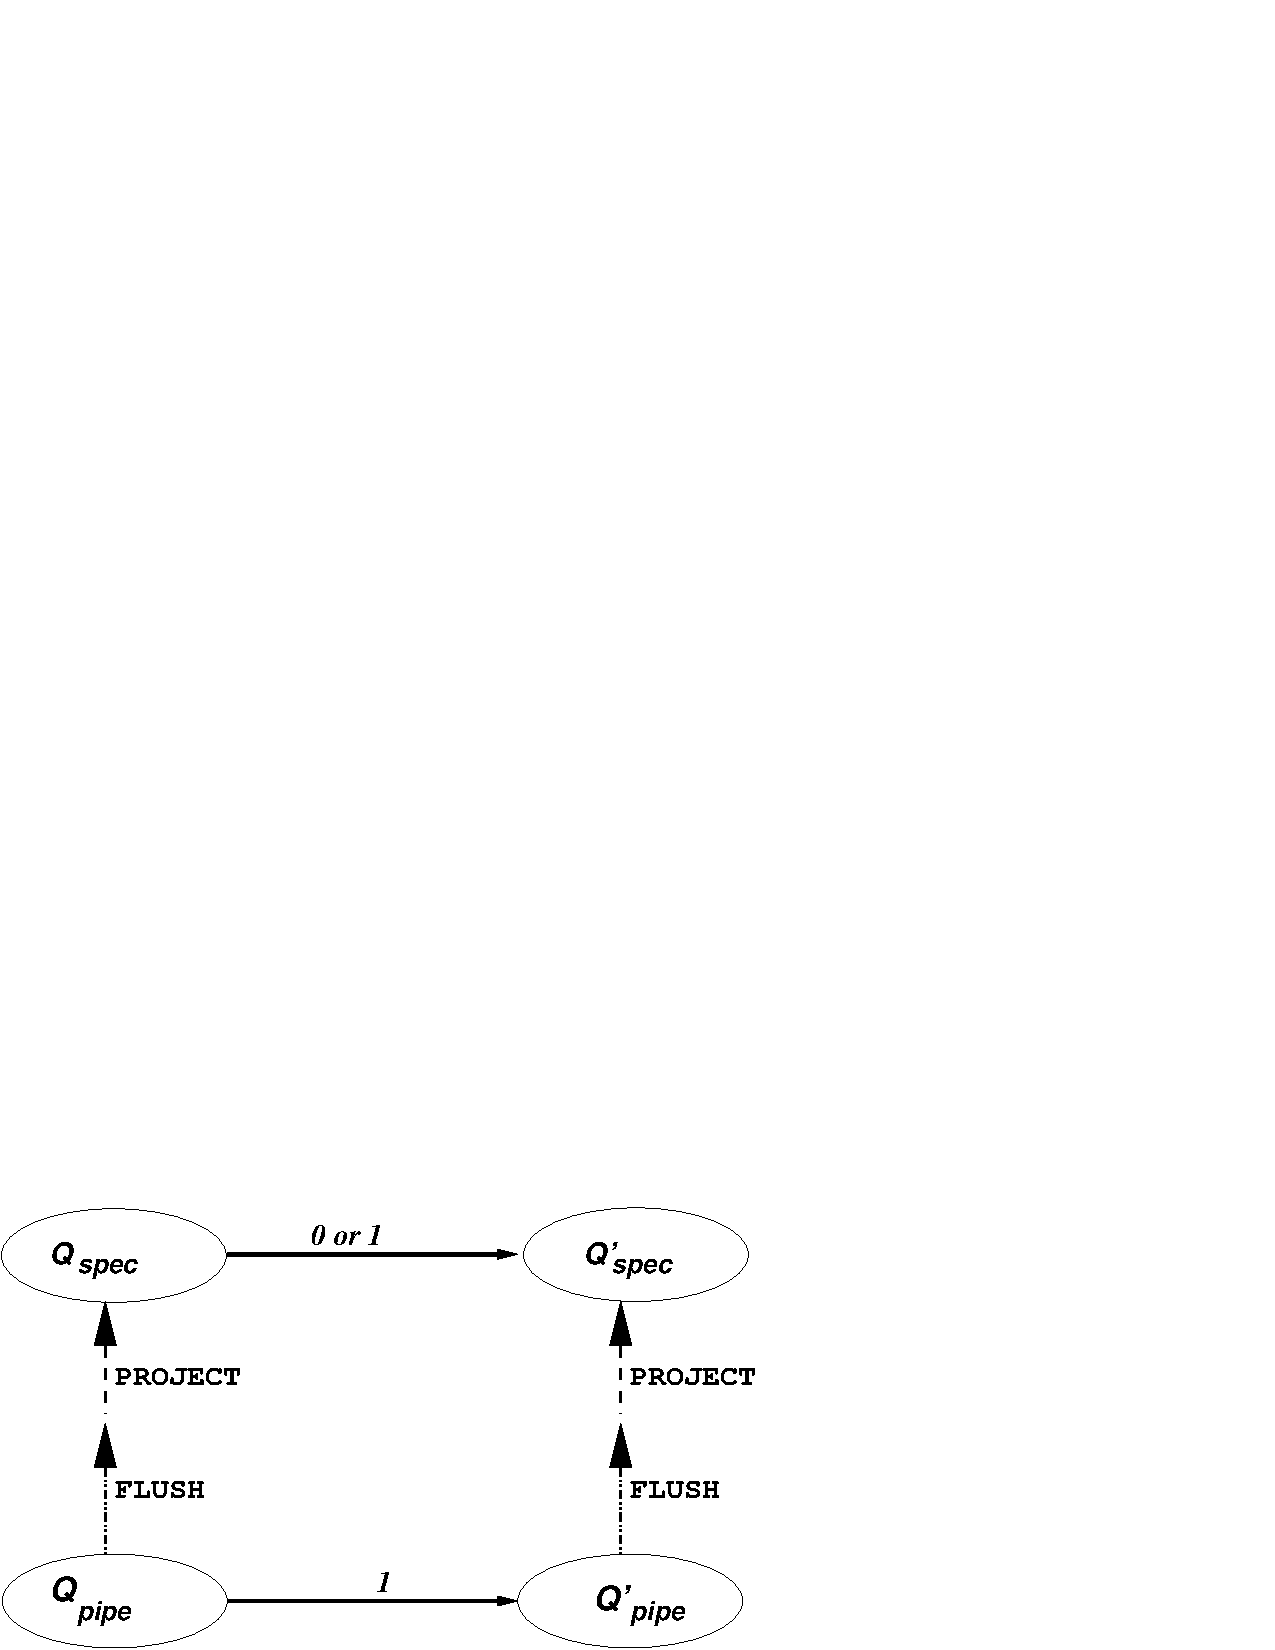
\includegraphics[width=0.7 \columnwidth]{figures/correspond.pdf}
   \label{fig:comm-diag}
	\caption{Commutative diagram to check an implementation (pipelined processor) is simulated by its specification.}
\end{figure}

Thus, the outline of the verification task, as
specified in the control section of a module,
involves simulating the two sides of the commutative (simulation)
diagram and checking an assertion at the end.
An example of correspondence checking, the verification of a simple
pipelined datapath,
is illustrated in detail in the code included below
(also in the distribution in \codelike{examples/simple-datapath.ucl}).
%Example~\ref{ex:simple-datapath}.
This example is drawn from the original UCLID system~\cite{DBLP:conf/cav/LahiriS04,bryant-cav02}.

%\begin{uclidlisting}[htbp]
    \lstinputlisting[language=uclid,style=uclidstyle]{../examples/simple-datapath.ucl}
%    \label{ex:simple-datapath}
%	\caption{\uclid{} model of a simple pipelined datapath in a processor, and verifying that it refines an instruction set architecture (ISA) level model.}
%\end{uclidlisting}


Running \uclid{} on the file given above produces the following output.
%Running \uclid{} on Example~\ref{ex:simple-datapath} produces the following output.

\begin{Verbatim}[frame=single, samepage=true]
$ uclid examples/simple-datapath.ucl
Successfully parsed 4 and instantiated 1 module(s).
10 assertions passed.
0 assertions failed.
0 assertions indeterminate.
Finished execution for module: main.
\end{Verbatim}

%---------------------------------------------------------
\section{Verifying Two-Safety Properties}

Certain security properties involve reasoning about a system
that is composed of modules modeling
multiple interacting agents, some of whom can be malicious. 
For confidentiality
properties, the goal is to ensure that secret data is not revealed to a malicious
agent. For integrity properties, the goal is that actions of a malicious agent
should not be able to influence the values of certain high-integrity variables.
Such properties form a special class of the general category of {\em hyperproperties}~\cite{clarkson-jcs10}
known as {\em $2$-safety properties}. The name arises from the way in which
such properties are checked, by formulating them as a safety property on a
``self-composed'' model of the system --- a model obtained by composing two
copies of the system together synchronously.

With \uclid{}, we verify $2$-safety properties via self-composition and
inductive invariant checking. Counterexamples comprise two traces
and are found by bounded model checking.
The code included below shows an
illustrative \uclid{} model drawn from the chapter on Security from the textbook
on embedded (cyber-physical) systems by Lee and Seshia~\cite{leeseshia-16}.

%\begin{uclidlisting}[htbp]
    \lstinputlisting[language=uclid,style=uclidstyle]{../examples/two-safety.ucl}
%    \label{ex:two-safety}
%	\caption{\uclid{} model of toy problem illustrating verification of two-safety properties}
%\end{uclidlisting}

%---------------------------------------------------------
\section{Synthesis}

\uclid{} has full support for Syntax-Guided Synthesis across all verification modes. If a synthesis function is inserted into the \uclid model, and the control block contains a verification command as per usual, \uclid{} will construct a synthesis query that searches for a body to any synthesis functions in the model. 

The example in Figure~\ref{fig:fib-induction-synth} uses synthesis to strengthen the invariant for the Fibonacci example we have seen before. When run with the command line option \codelike{-y "cvc5 --lang=sygus2"} (or another SyGuS solver), \uclid{} will return the correct body for the synthesis function so that the verification condition passes.

\begin{uclidlisting}[htbp]
    \lstinputlisting[language=uclid,style=uclidstyle]{../examples/fib2safety-synth.ucl}
    \caption{\uclid{} Fibonacci model using \codelike{synthesis function}}
    \label{ex:fib-induction-synth}
\end{uclidlisting}




\bibliographystyle{plain}
\bibliography{refs}

\appendix
\chapter{Appendix: \uclid{} Grammar}

\newcommand{\paratitle}[1]{\textsf{\textbf{#1}}}
\newcommand{\nonterminal}[1]{$\langle \textit{#1} \rangle$}

\setlength{\grammarindent}{12em} % increase separation between LHS/RHS 

This appendix describes \uclid{}'s grammar.

\section{Grammar of Modules and Declarations}
\paratitle{A model} consist of a list of modules. Each module consists of a list of declarations followed by an optional control block.
\begin{grammar}
     <Model> ::= <Module>*

     <Module> ::= \keywordbf{module} <Id>~~ `{' <Decl>* <ControlBlock>? `}'
\end{grammar}

\paratitle{Declarations} can be of the following types.
\begin{grammar}
     <Decl> ::= <TypeDecl> 
            \alt <InputsDecl> 
            \alt <OutputsDecl> 
            \alt <VarsDecl> 
            \alt <SharedVarsDecl> 
            \alt <DefineDecl>
            \alt <ConstsDecl> 
            \alt <ConstLitDecl>
            \alt <FuncDecl> 
            \alt <ProcedureDecl> 
            \alt <InstanceDecl>
            \alt <InitDecl> 
            \alt <NextDecl> 
            \alt <AxiomDecl>
            \alt <SpecDecl> 
\end{grammar}

\paratitle{Type declarations} declare either a type synonym or an uninterpreted type.
\begin{grammar}
     <TypeDecl> ::= \keywordbf{type} <Id> `=' <Type> `;'
              \alt \keywordbf{type} <Id> `;'

\end{grammar}

\paratitle{Variable declarations} can refer to inputs, outputs, state variables, symbolic constants, named constant literals, shared variables, group declarations, or define declarations.
\begin{grammar}
     <InputsDecl> ::=
       \keywordbf{input} ~ <IdList> `:' <Type> `;'

     <OutputsDecl> ::=
       \keywordbf{output} ~ <IdList> `:' <Type> `;'

     <VarsDecl> ::=
       \keywordbf{var} ~ <IdList> `:' <Type> `;'

     <ConstsDecl> ::=
       \keywordbf{const} ~ <IdList> `:' <Type> `;'

     <ConstLitDecl> ::=
       \keywordbf{const} ~ <Id> ~ `:' <Type> = <Number> `;'

     <SharedVarsDecl> ::=
       \keywordbf{sharedvar} ~ <IdList> `:' <Type> `;'

     <DefineDecl> ::= 
       \keywordbf{define} <Id> `(' <IdTypeList> `)' `:' <Type> `=' <Expr>  `;'

     <GroupDecl> ::= 
       \keywordbf{group}~ <Id> ~`:' <Type> `=' <IdList> `;'

\end{grammar}

\paratitle{Function declarations} refer to uninterpreted functions, synthesis functions or oracle functions. 
\begin{grammar}
     <FuncDecl> ::= 
       \keywordbf{function} <Id> `(' <IdTypeList> `)' `:' <Type> `;'

     <SynthFuncDecl> ::= 
       \keywordbf{synthesis} \keywordbf{function} <Id> `(' <IdTypeList> `)' `:' <Type> `;'

     <OracleFuncDecl> ::= 
       \keywordbf{oracle} \keywordbf{function} <Id> <AnnotationList> `(' <IdTypeList> `)' `:' <Type> `;'

\end{grammar}

\paratitle{Procedure declarations} consist of a formal parameter list, a list of return values and types, 
followed by optional pre-/post-conditions and the list of state variables modified by procedure.
\begin{grammar}
     <ProcedureDecl> ::=
       \keywordbf{procedure} <Id> (<AnnotationList>)* `(' <IdTypeList> ')' <ProcReturnArg>? \\
       <RequireExprs> <EnsureExprs> <ModifiesExprs> \\
       <BlkStmt>

     <ProcReturnArg> ::= \keywordbf{returns} `(' <IdTypeList> `)'

     <RequireExprs> ::= ( \keywordbf{requires} <Expr> `;' )*

     <EnsureExprs> ::= ( \keywordbf{ensures} <Expr> `;' )*

     <ModifiesExprs> ::= ( \keywordbf{modifies} <IdList> `;' )*

\end{grammar}

\paratitle{Instance declarations} allow the instantiation (duh!) of other modules. They consist of the instance name, the name of the module being instantiated and the list of mappings for the instances' inputs, output and shared variables. 
\begin{grammar}
     <InstanceDecl> ::= \keywordbf{instance} <Id> `:' <Id> <ArgMapList> `;'

     <ArgMapList>   ::= `(' `)' 
                    \alt `(' <ArgMap> `,' <ArgMapList> `)'

     <ArgMap> ::= <Id> `:' `(' `)' 
              \alt <Id> `:' `(' <Expr> `)'
             
\end{grammar}

\paratitle{Axioms} refer to assumptions while a \paratitle{specification declaration} refers to design \keywordbf{invariants}. Note \keywordbf{axiom} and \keywordbf{assume} are synonyms, as are \keywordbf{property} and \keywordbf{invariant}.

\begin{grammar}
     <AxiomDecl> ::= <AxiomKW> <Id> `:' <Expr> `;'
                 \alt <AxiomKW> <Expr> `;'

     <AxiomKW> ::= \keywordbf{axiom} | \keywordbf{assume}

     <SpecDecl> ::= <PropertyKW> <Id> `:' <Expr> `;'
                 \alt <PropertyKW> <Expr> `;'

     <PropertyKW> ::= \keywordbf{property} | \keywordbf{invariant}
\end{grammar}

\paratitle{Init} and \paratitle{next} blocks consist of lists of statements.
\begin{grammar}
     <InitDecl> ::= \keywordbf{init} <BlkStmt>

     <NextDecl> ::= \keywordbf{next} <BlkStmt>

\end{grammar}
Assignment statements in the \keywordbf{next} block declaration must
assign primed variables only, and are concurrently evaluated.

\section{Statement Grammar}
\paratitle{Statements} are the following types, most of which should be familiar. Note the support for simultaneous assignment \`a la Python. The keyword \keywordbf{next} allows for synchronous scheduling of instantiated modules.
\begin{grammar}
     <Statement> 
       ::= \keywordbf{skip} `;' 
       \alt \keywordbf{assert} <Expr> `;'
       \alt \keywordbf{assume} <Expr> `;'
       \alt \keywordbf{havoc} <Id>  `;'
       \alt <LhsList> `=' <ExprList> `;'
       \alt \keywordbf{call} `(' <LhsList> `)' `=' <Id> <ExprList> `;'
       \alt \keywordbf{call} <Id> `(' <ExprList> `)' `;'
       \alt \keywordbf{next} `(' <Id> `)' `;'
       \alt <IfStmt>
       \alt <CaseStmt>
       \alt <ForLoop>
       \alt <WhileLoop>
       \alt <BlkStmt>
\end{grammar}

\paratitle{Block statements} are a list of variables with local scope, and a list of statements.

\begin{grammar}
    <BlkStmt> ::= `{' <BlockVarDecl>* <Statement>* `}'

    <BlockVarDecl> ::= \keywordbf{var} <IdList> `:' <Type> `;'
\end{grammar}


\paratitle{Assignments} and \paratitle{call} statements refer to the nonterminal \nonterminal{LhsList}. As the name suggests, this is a list of syntactic forms that can appear on the left hand side of an assignment. \nonterminal{Lhs} are of four types: (i) identifiers, bitvector slices within identifiers, (iii) array indices, and (iv) fields within records.
\begin{grammar}
    <LhsList> ::= <Lhs> (`,' <Lhs>)*

    <Lhs> ::= <Id>
	  \alt <Id> `'' 
          \alt <Id> `[' <Expr> `:' <Expr> `]'
          \alt <Id> `[' <ExprList> `]'
          \alt <Id> (`.' <Id>)+
\end{grammar}

\paratitle{If} statements are as per usual. ``Braceless'' if statements are not permitted.
\begin{grammar}
    <IfStmt> ::= 
    \keywordbf{if} `(' <CondExpr> `)'  <BlkStmt> \\ \keywordbf{else} <BlkStmt>
    \alt \keywordbf{if} `(' <CondExpr> `)'  <BlkStmt>

    <IfExpr> ::= <Expr> | *
\end{grammar}

\paratitle{Case} statements are as follows.
\begin{grammar}
    <CaseStmt> ::= \keywordbf{case} <CaseBlock>* \keywordbf{esac}

    <CaseBlock> ::= <Expr> `:' <BlkStmt>
                \alt \keywordbf{default} `:' <BlkStmt>
\end{grammar}

\paratitle{For loops} allow iteration over a statically defined range of values.
\begin{grammar}
    <ForLoop> ::= \keywordbf{for} <Id> \keywordbf{in} \keywordbf{range} `(' <Number> ',' <Number> `)' \\
                  <BlkStmt>
\end{grammar}

\paratitle{While loops} allow unbounded iteration.
\begin{grammar}
    <WhileLoop> ::= \keywordbf{while} `(' <CondExpr> `)' \\
                  <InvariantClause>* \\
                  <BlkStmt>

    <InvariantClause> ::= \keywordbf{invariant} <Expr> `;'
\end{grammar}

\section{Expression Grammar}
Let us turn to \paratitle{expressions}, which may be quantified (include finite forall quantifiers, which expand to a disjunction and quantify over a finite group). 
\begin{grammar}
    <Expr> ::= <E1>

    <E1> ::= <E2>
         \alt `(' \keywordbf{forall} `(' <IdTypeList> `)' `::' E1 `)'
         \alt `(' \keywordbf{exists} `(' <IdTypeList> `)' `::' E1 `)'
         \alt `(' \keywordbf{finite_forall} `(' <GroupDecl> `)' `::' E1 `)'

\end{grammar}

The usual logical and bitwise operators are allowed.
\begin{grammar}
    <E2> ::= <E3> `<==>' <E2> | <E3>

    <E3> ::= <E4> `==>' <E3> | <E4>

    <E4> ::=  <E5> `&&' <E4> | <E5> `||' <E4> | 
         \alt <E5> `&' <E4> | <E5> `|' <E4> | <E5> `^' <E4> 
         \alt <E5>
\end{grammar}

As are relational operators, bitvector concatentation (++) and arithmetic.

\begin{grammar}
<E5> ::=  <E6> <RelOp> <E6> | <E6>

<RelOp> ::= `>' | `<' | `=' | `!=' | `>=' | `<='

<E6> ::=  <E7> `++' <E6> | <E7>

<E7> ::=  <E8> `+' <E7> | <E8>

<E8> ::=  <E8> `-' <E9> | <E9>

<E9> ::= <E9> `*' <E10> | <E9> `/' <E10> | <E10>
\end{grammar}

The unary operators are arithmetic negation (unary minus), logical negation and bitwise negation of bitvectors.
\begin{grammar}
    <E10> ::= <UnOp> <E11> | <E11>

    <UnOp> ::= `-' | `!' | `~'
\end{grammar}

Array select, update and bitvector select operators are defined as follows.
\begin{grammar}
    <E11> ::= <E12> `[' <Expr> (`,' <Expr>)* `]'
          \alt <E12> `[' <Expr> (`,' <Expr>)* `->' <Expr> `]'
          \alt <E12> `[' <Expr> `:' <Expr> `]'
          \alt <E12>
\end{grammar}

Function invocation, record selection, and access to variables in instantiated modules is as follows.
\begin{grammar}
    <E12> ::=  <E13> `(' <ExprList> `)'
          \alt <E13> (`.' <Id>)+
\end{grammar}

And finally, we have the terminal symbols, identifiers, record field access, tuples and the if-then-else operator.
\begin{grammar}
    <E12> ::= \keywordbf{false} | \keywordbf{true} | <Number> | <String>
          \alt <Id> | <Id> `.' <Id>
          \alt `{' <Expr> (`,' <Expr>)* `}'
          \alt \keywordbf{if} `(' <Expr> `)' \keywordbf{then} <Expr> \keywordbf{else} <Expr>
\end{grammar}

Strings can only be used as arguments to the \texttt{print} command in the control block.

\section{Types}

\begin{grammar}
<Type> ::= <PrimitiveType> 
       \alt <EnumType> 
       \alt <TupleType> | <RecordType> 
       \alt <ArrayType> 
       \alt <SynonymType> 
       \alt <ExternalType> 
%%     }
\end{grammar}

Supported primitive types are Booleans, integers, floats and bit-vectors. Bit-vector types are defined according the regular expression `bv[0-9]+' and the number following `bv' is the width of the bit-vector.

\begin{grammar}
    <PrimitiveType> ::= \keywordbf{boolean} | \keywordbf{integer} | <FloatType> | <BitVectorType>
\end{grammar}

Enumerated types are defined using the \keywordbf{enum} keyword.
\begin{grammar}
    <EnumType> ::= \keywordbf{enum} `{' <IdList> `}'
\end{grammar}

Tuple types are declared using curly brace notation.
\begin{grammar}
    <TupleType> ::= `{' <Type>  (`,' <Type>)* `}'
\end{grammar}

Record types use the keyword \keywordbf{record}.
\begin{grammar}
    <Recordtype> ::= \keywordbf{record} `{' <IdTypeList> `}'
\end{grammar}

Array types are defined using square brackets. The list of types within square brackets defined the array's index type.
\begin{grammar}
    <ArrayType> ::= `[' <Type> (`,' <Type>)* `]' <Type>
\end{grammar}


Type synonyms are just identifiers, while external types refer to synonym types defined in a different module.
\begin{grammar}
    <SynonymType> ::= <Id>

    <ExternalType> ::= <Id> `.' <Id>
\end{grammar}

\section{Control Block}
\paratitle{The control block} consists of a list of commands. A command can have an optional result object, an optional argument object, an optional list of command parameters and finally an optional list of argument expressions. 
\begin{grammar}
     <ControlBlock> ::= \keywordbf{control}~~ `{' <Cmd>* `}'

     <Cmd> ::= (<Id> `=' )? (<Id> `.')? <CmdName> \\
              (`[' <IdList> `]')? <ExprList>? `;'
\end{grammar}


The following is a list of currently accepted commands.

\begin{grammar}
    <CmdName> ::= `bmc' \alt
                  `bmc_LTL' \alt
                  `bmc_noLTL' \alt
                  `check' \alt
                  `clear\_context' \alt
                  `induction' \alt
                  `print' \alt
                  `print\_cex' \alt
                  `print\_module' \alt
                  `print\_results' \alt
                  `print\_smt2'
                  `unroll' \alt
                  `verify'
\end{grammar}

\section{Miscellaneous Nonterminals} 

\nonterminal{IdList}, \nonterminal{IdTypeList} and \nonterminal{ExprList} are non-empty, comma-separated list of identifiers, identifier/type tuples and expressions respectively.
\nonterminal{AnnotationList} is a non-empty comma-separated list of strings, used as annotations to indicate, for example, whether a procedure should be inline or not.
\begin{grammar}
     <IdList> ::= <Id> \alt <Id> `,' <IdList>

     <IdTypeList> ::=  <Id> (`,' <Id>)* `:' <Type> 
                  \alt <Id> (`,' <Id>)* `:' <Type> `,' <IdTypeList>

     <ExprList> ::=  <Expr>
                \alt <Expr> `,' <ExprList>

     <AnnotationList> ::= `[' <String> (`,' <String>)*`]'          
\end{grammar}




\end{document}
